% !TeX root = cluster.tex
\documentclass[paper.tex]{subfiles}

\begin{document}
	\section{Determining the Aggregation Function $A$}
	
	At first glance, the ranking of the variables $\V$ seems entirely subjective. It's not hard to buy that this aggregation function $A$ depends on the given variables, but the manner in which each variable ``positively impacts student performance'' is very dependent on what it actually \emph{means}. Unfortunately for us, the semantics of the data depend on world knowledge tied into the description, and there's no intrinsic reason to prefer any given variables over any other.
	
	Nonetheless, we might be able to exploit internal consistencies in the data to absolve ourselves of needing to manually assign ``goodness'' values to every variable. The idea is as follows: even without knowing anything about what variables do, we might be able to group them by how co-variate they are. Then, we assign each of those groupings some sort of semantics, assume that we can use the covariance of the variables as a way to carry the broad semantic interpretation back to the uninterpreted data. Even so, we haven't quite managed to escape the fact that we're building a subjective semantics from incomplete data; instead, we have subtly replaced some subjectivity with a handful of relatively palatable assumptions: 
	\begin{enumerate}
		\item The co-variance of two variables is meaningful because we humans have subconsciously picked variables that over-represent the things that we know.
		\item The distance metric is nicely behaved -- i.e., two semantically equivalent variables align well in our data, and two disparate variables have good separation.
		\item As a result, we can follow the ``centers'' of these groups nicely back into the data to find the centers of semantic categories we care about.
		\item Student success is a quantity which widely influences many of these variables.
	\end{enumerate} 
	If you're wondering why you should buy those assumptions -- it's not because they're defensible, but because they are succinct and there aren't very many of them -- very much unlike the case in which we manually assign each of the variables a weight. The point is that we don't really know what we're doing, and hope is that if we give a computer a little nudge in the right direction, it will find better weights than we ourselves could come up with. This turns out to be a common objective -- there is an entire sub-discipline of Machine Learning focused on leaning functions without any labeled examples (unsupervised) or with very few examples (weakly supervised). In both cases, the aim is to exploit internal consistencies in data.
	
	\subsection{Clustering}
	We used the lovely \texttt{scikit-learn} library to do the clustering for us -- 
	
	Normally, a clustering algorithm looks at a set of samples
	
	
	\subsection{Semantic Trees}
	
	\subsection{Clustering Results}
	The K-Means and Feature Agglomeration
	
	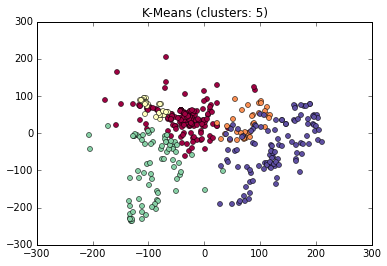
\includegraphics[width=0.5\linewidth]{images/clusters_km_5.png}
	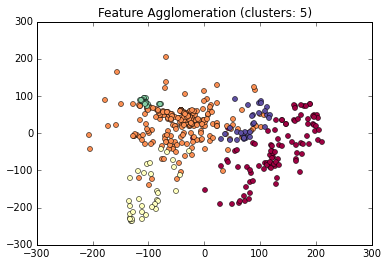
\includegraphics[width=0.5\linewidth]{images/clusters_fa_5.png}
		
	\subsection{Models to Assign Weights}
	The simplest model to consider is a linear one:
	\[A(v) = \sum_i a_i v_i \]
	
\end{document}